\subsection{Three-phase Electric Power}
\begin{define}
    \textbf{Three-phase electric power:} a common type of alternating current (AC) used in electricity generation, transmission, and distribution. Typically employs 3-4 wires (fourth wire is an optional neutral return wire).

    \textbf{Line voltage:} the voltage between any two lines

    \textbf{Phase voltage:} the voltage measured between any line and neutral
\end{define}
This three-phase electric power is a common method used by electrical grids to transfer power. The voltage on each wire is 120$^\circ$ phase shifted from each other. This allows voltages to be stepped up using transformers to high voltage and stepped down for distribution. Each conductor in a \textit{symmetric} three-phase power supply system carries an alternating current of the same frequency and voltage amplitude. You can design assymetric three-phase power systems, but are not used in practice.

Convention states that for a 208/120-volt service, that means that the line voltage is 208 volts and the phase voltage is 120 volts.

\subsubsection{Advantages}
If we had to compare a three-phase supply to a single phase AC power supply (with two current-carrying conductors, phase and neutral), a three-phase supply with no neutral and the same phase-to-ground voltage/current capacity per phase would transmit 3 times as much power with only 1.5 imes as much wires (3 vs 2 wires). This means that we get higher efficiency, lower weight, and cleaner waveforms.

Here are more properties of three-phase supplies that are desirable in electric power systems:
\begin{itemize}
    \item Phase currents tend to cancel each other out, summing to 0 in a linear balanced load. Due to this, sometimes we don't even need a neutral conductor since it will carry little or no current.
    \item Power transfer into a linear balanced load is constant, which helps to reduce vibrations in motor/generators
    \item Can produce a rotating magnetic field with a specificed direction and constant magnitude. This simplifies the design of electric motors since no starting circuit is required
\end{itemize}

\subsubsection{Disadvantages or Cautions}
Make sure that the phases are connected in the correct order to achieve the intended direction of rotation of three-phase motors. If two sources are connected at the same time, then a direct connection between two different phases is a short circuit and leads to flow of unbalanced current.

\subsubsection{Why not a higher number of phases?}
Three phases is the minumum number that we can have without having "dead" spots in the cycle.

Industry uses almost exclusively three phase power since an induction motor needs at least a three phase supply to start and run in a known direction. Single phase induction motors require lossy, unreliable, and expensive tricks to do the same (extra windings, lossy windings, speed sensitive switch, capacitors, etc).

The supply grid is based on three phase since that is the most efficient in terms of generation and delivery. Using a 9 phase grid for example would require running 9 wires for the entire distribution grid, not cost effective.

The higher order motors mentioned don't use line generated phases. Stepper motors use more phases for finer control. High order polyphase rectifiers are designed often with more 'phases', to reduce ripple, but the phases are generated locally by phase-shifting the line input by some means, either direct LC shifting, or by using a motor-generator set.

Mathematically there is no improvement in motor smoothness, 3 is already an optimal case.

\subsubsection{Delta and Wye}
There are two basic three-phase configurations
\begin{define}
    \begin{center}
        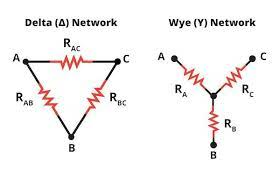
\includegraphics[scale=0.8]{figs/delta_wye.jpeg}
    \end{center}
\end{define}

For a $\wye$ configuration, there is an optional fourth wire, which serves as a neutral and is normally grounded. The ground wire present above many transmission lines are for fault protection and doesn't carry current under normal use.

There are four different types of three-phase transformer winding connections for transmission and distribution.
\begin{enumerate}
    \item $\wye - \wye$: for small current and high voltage
    \item $\Delta - \Delta$: for large currents and low voltages
    \item $\Delta - \wye$: for step-up transformers (ie generating stations)
    \item $\wye - \Delta$: for step-down transformers (ie at end of the transmission)
\end{enumerate}

\begin{figure}[H]
    \centering
    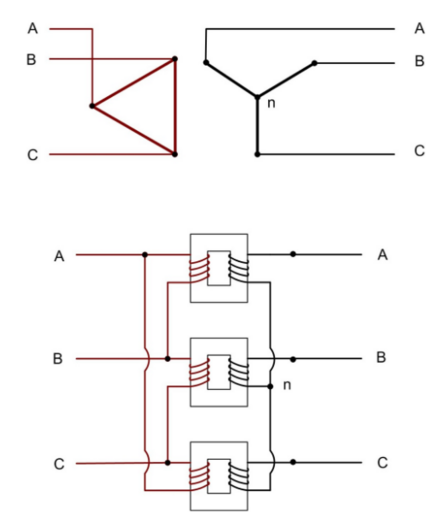
\includegraphics[scale=0.5]{figs/Delta-Wye_Transformer.png}
    \caption{This shows a delta-wye configuration across a transformer core. A practice transformer wouldn't have a different number of turns on each side.}
\end{figure}